%%%%%%%%%%%%%%%%%%%%%%%%%%%%%%%%%%%%%%%%
% PDF compatibility code. 
\makeatletter
\newif\ifpdflatex@
\ifx\pdftexversion\@undefined
\pdflatex@false
%\message{Not using pdf}
\else
\pdflatex@true
%\message{Using pdf}
\fi

\newcommand{\latexorpdf}[2]{
  \ifpdflatex@ #2
  \else #1
  \fi
}

\makeatother

#ifdef A4Format
\newcommand{\pformat}{a4paper}
#endif A4Format
#ifdef LetterFormat
\newcommand{\pformat}{letterpaper}
#endif LetterFormat

%%%%%%%%%%%%%%%%%%%%%%%%%%%%%%%%%%%%%%%%

\latexorpdf{
\documentclass[\pformat,11pt]{article}
}{
\documentclass[\pformat,pdftex,11pt]{article}
}

\usepackage[dvipdfm]{graphicx, color}
\usepackage[dvipdfm,bookmarks=true,bookmarksnumbered=true,colorlinks,plainpages=true]{hyperref}

\usepackage{toolbox}
\usepackage{vdmsl-2e}
\usepackage{makeidx}
\usepackage{alltt}
%\usepackage{graphics}
%\usepackage{verbatim}
\usepackage{ifthen}
\usepackage{verbatimfiles}
%\usepackage{color}
\usepackage{longtable}
\usepackage{tabularx}
\usepackage{here}
\usepackage{moreverb}
\usepackage{subfig}

\graphicspath{{figures/}}
\def\seename{$\Rightarrow$}

%\usepackage{psboxit}
%\PScommands
\setlength{\fboxrule}{0pt}
\setlength{\fboxsep}{1pt}

\newlength{\negoneline}
\addtolength{\negoneline}{-11pt}

\newcommand{\listingsize}[0]{\renewcommand{\baselinestretch}{0.95}\tt\footnotesize}

\newcommand{\startbox}[0]{
\begin{center}
\listingsize  
\begin{tabular}{|p{.975\textwidth}|}\hline\vspace{\negoneline}}
\newcommand{\interruptbox}[0]{
\end{tabular}
\end{center}}

\newcommand{\keyw}[1]{{\sf #1}}

\newcommand{\continuebox}[0]{
\begin{center}
\listingsize  
\begin{tabular}{|p{.975\textwidth}|}\vspace{\negoneline}}

\newcommand{\closebox}[0]{
\\\lasthline
\end{tabular}
\end{center}}

\newcommand{\scriptlistingsize}[0]{\tt\scriptsize}

%\newcommand{\gbx}[1]{\psboxit{ box .75 setgray fill}{\spbox{#1}}}
\definecolor{bggray}{gray}{.80}
\newcommand{\gbx}[1]{\colorbox{bggray}{#1}}

%\usepackage{path}

% Ueki change start
\usepackage[dvipdfm,bookmarks=true,bookmarksnumbered=true,colorlinks,plainpages=true]{hyperref}
% Ueki change end

% Ueki delete start
%\latexorpdf{
%\usepackage[plainpages=true,colorlinks,linkcolor=black,citecolor=black,pagecolor=black, urlcolor=black]{hyperref}
%}{
%\usepackage[plainpages=true,colorlinks]{hyperref}
%}
% Ueki delete end

\makeindex

%\parindent0mm

\def\insertfig#1#2#3#4{ % Filename, width, caption, label
\begin{figure}[H]
\begin{center}
\epsfig{file=#1,width=#2,angle=-90}
\end{center}
\caption{#3} #4
\end{figure} 
}
\def\insertfigx#1#2#3#4{ % Filename, width, caption, label
\begin{figure}[H]
\begin{center}
\epsfig{file=#1,width=#2}
\end{center}
\caption{#3} #4
\end{figure} 
}
\newcommand{\vdmslpp}{VDM++}
\newcommand{\vdmslppEm}{VDM\/++}
\newcommand{\ToolboxName}{VDM++ Toolbox}
\newcommand{\Toolbox}{Toolbox}
\newcommand{\toolbox}{toolbox}
\newcommand{\vdmde}{vppde}
\newcommand{\vdmgde}{vppgde}
\newcommand{\vdmhome}{vpphome}
\newcommand{\vdmdeNineteen}{vppde-19}
\newcommand{\vdmdeNineteenEl}{vppde-19.el}
\newcommand{\tcg}{the Code Generator}
\newcommand{\Tcg}{The Code Generator}
\DeclareRobustCommand{\VdmSlPp}{VDM++-\VdmSl}
\newcommand{\libmancite}{\cite{LibMan-SCSK}}
\newcommand{\langmancite}{\cite{LangManPP-SCSK}}
\newcommand{\VDM}{VDM++}
\newcommand{\cg}{VDM++ to Java Code Generator}
\newcommand{\ccg}{Concurrent \cg}
\newcommand{\JL}{VDM Java Library}
\newcommand{\CJL}{Concurrent VDM Java Library}
\newcommand{\CGBase}{\texttt{CGBase}}

\newcommand{\guicmd}[1]{{\sf #1}}

\begin{document}

\vdmtoolsmanualscsk{
#ifdef VICEMAN
  The VDM++ VICE to Java Code Generator
#else
  The VDM++ to Java Code Generator
#endif VICEMAN
  }
  {2.0}

\section{Introduction}

The \cg\ supports automatic generation of Java code from \VDM\ 
specifications. \Tcg\ provides a rapid way of 
implementing Java applications based on \VDM\ specifications.

\Tcg\ is an add-on feature to the \ToolboxName{}. This manual
is an extension to the {\em User Manual for the \VDM{} Toolbox}
\cite{UserManPP-SCSK} and gives an introduction to the \cg{}. 

This manual is structured in the following way:

Section~\ref{invoking} gives an introduction to the \cg{}. It
describes how to invoke the Code Generator from the \ToolboxName{} and
provides guidance on interfacing the generated Java
code. Furthermore, it will be explained how to compile and run the
Java code. 

Section~\ref{advancedissues} presents four more advanced issues. It
summarizes the options which can be chosen when generating Java code
from \VDM\ specifications. Moreover, it describes how to handle
implicit or preliminary function/operation definitions and it
discusses the possibilities for substituting generated Java code with
handwritten code. Finally, it will list the requirements which a \VDM\
specification must fulfil in order to be translated to compilable and
correct Java code. 

Section~\ref{sec:relation} gives a detailed description of the
structure of the generated Java code. In addition, it explains the
relation between \VDM\ and Java data types, and it describes some of
the design decisions made, when developing the \cg{}, including the
name conventions used. This section should be studied intensively
before using \tcg\ professionally.

Finally, in Section~\ref{concmain} an explanation of how to generate
code for concurrent specifications is provided. For such
specifications, multithreaded Java code is generated. As well
as instructions on use, an overview of the translation approach is given. 
\newpage

\section{The Code Generator - Getting Started}\label{invoking}

To get started using \tcg\ a \VDM\ specification should be written in
one or several files. 

In the following, the \VDM\ specification of a class {\tt DoSort} will
be used in order to illustrate the Java Code Generator.  The
specification is listed in Appendix \ref{sec:vdmDoSort} and it can be
found in file {\tt Sort.rtf} provided in the distribution. 
In Section~\ref{gui} it is explained how to generate Java code for the
\VDM\ {\tt DoSort} class using the \ToolboxName{}. In
Section~\ref{interfacinggettingstarted} it is explained how to
write an application on top of the generated Java code. In
Section~\ref{compileandrun} it is shown how to compile and run
the application. 

It is recommended that readers go through the steps described in
Section~\ref{gui} to ~\ref{compileandrun} on their own computer.

\subsection{Generating Code Using the VDM++ Toolbox}\label{gui}

We will now describe how to use the \cg\ from the graphical user
interface of the \ToolboxName{}. 

Having started the \ToolboxName{}, a new project should be created the
{\tt Sort.rtf} file. Before generating Java code, it has to be
ensured, that the \VDM\  specification satisfies the necessary
requirements: 

\begin{itemize}
\item
{\em All} files of the \VDM\ specification in a project must have
successfully been syntax checked in order to generate correct code
for any selected class.  

\item
Moreover, \tcg\ can only generate code for classes which are type
correct.\footnote{There exist two classes of well-formedness as
  explained in \langmancite. In the current context we mean possible
  well-formed type correctness.} If a class has not been type checked
before and one tries to generate code for it, it is automatically type
checked by the \Toolbox{}.  
\end{itemize}

Syntax and type check the {\tt DoSort} class as described in the {\em
  User Manual for the \VDM{} Toolbox} \cite{UserManPP-SCSK}. The
  result is shown in Figure~\ref{fig:toolbox}. 

\begin{figure}[H]
\begin{center}
\mbox{}
\resizebox{9.2cm}{!}{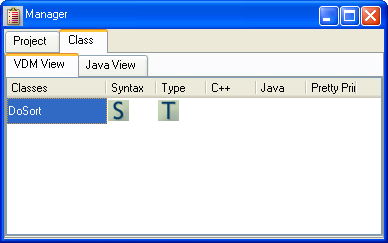
\includegraphics{toolbox}}
\caption{The Manager after Syntax and Type Checking}\label{fig:toolbox}
\end{center}
\end{figure}

You can now generate code for the {\tt DoSort} class by clicking on
the \raisebox{-1.0mm}{
\includegraphics[width=0.03\textwidth]{java}}
(\guicmd{Generate Java}) button. In general, more than one file/class
can be selected, in which case all of them are translated to Java.

Figure~\ref{fig:interpreter} shows how to generate Java code for the
{\tt DoSort} class.  As can be seen, a Java file called {\tt
  DoSort.java} has been code generated.  It contains the Java class
definition of {\tt DoSort}.  The {\tt DoSort.java} file will be written in the
directory, where the project file lies. If no project file exists, the
file will be written in the directory, where the VDM++ Toolbox was
started.

Figure~\ref{fig:vdmjava} shows a skeleton of the VDM++ specification
and the corresponding generated Java code for class {\tt DoSort}.  The
different parts of the generated code will be explained in the
following sections. The file {\tt DoSort.java} is shown in full in
Appendix \ref{sec:javaDoSort}. 

\begin{figure}[H]
\begin{center}
\mbox{}
\resizebox{9.2cm}{!}{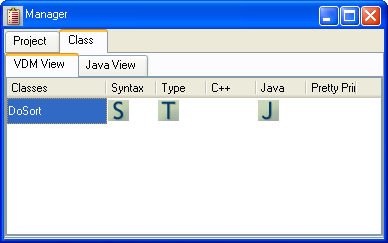
\includegraphics{dosort}}
\caption{Code generating the {\tt DoSort} class.}\label{fig:interpreter}
\end{center}
\end{figure}

\begin{figure}
\begin{center}
%\begin{minipage}[t]{2.5in}
\begin{quote}
\begin{small}
\begin{verbatim}  
class DoSort

operations
  public Sort: seq of int ==> seq of int
  Sort(l) ==
    ...

functions

  protected DoSorting: seq of int -> seq of int
  DoSorting(l) ==
    ...

  private InsertSorted: int * seq of int -> seq of int
  InsertSorted(i,l) ==
    ...

end DoSort
\end{verbatim}
\end{small}
\end{quote}
%\end{minipage} 
VDM++ 
%\begin{minipage}[t]{2.5in}
%\vspace{2cm}
\begin{quote}
\begin{small}
\begin{verbatim}  
public class DoSort {

// ***** VDMTOOLS START Name=vdmComp KEEP=NO
  static UTIL.VDMCompare vdmComp = new UTIL.VDMCompare();
// ***** VDMTOOLS END Name=vdmComp


// ***** VDMTOOLS START Name=Sort KEEP=NO
  public Vector Sort (final Vector l) throws CGException{
    ...
  }
// ***** VDMTOOLS END Name=Sort


// ***** VDMTOOLS START Name=DoSorting KEEP=NO
  protected Vector DoSorting (final Vector l) throws CGException{    
    ...
  }
// ***** VDMTOOLS END Name=DoSorting


// ***** VDMTOOLS START Name=InsertSorted KEEP=NO
  private Vector InsertSorted (final Long i, final Vector l) 
                              throws CGException {    
    ...
  }
// ***** VDMTOOLS END Name=InsertSorted
}
\end{verbatim}
\end{small}
\end{quote}
%\end{minipage}
%Java
\caption{The VDM++ and the generated Java {\tt DoSort} class.\label{fig:vdmjava}}
\end{center}
\end{figure}


It is also possible to generate Java code from the command-line
version of the \ToolboxName. The \ToolboxName\ is started from the
command line with the command {\tt
\vdmde}\index{vdmde!starting}. The {\tt -j} option is used in order to
generate Java code. To code generate the class {\tt DoSort},
the following command is executed:

\begin{quote}
\begin{verbatim}
vppde -j Sort.rtf
\end{verbatim}
\end{quote}

The specification will be parsed first. If no syntax errors are
detected, the specification will be type checked for possible
well-formedness. Finally, if no type errors are detected, the
specification will be translated into a number of Java files.  For the
described specification, the file {\tt DoSort.java} containing the
{\tt DoSort} class definition will be generated.

Note: If a specification contains several classes and the command-line
version of \Tcg\ is used, all classes have to be code generated at the
same time.

%For each \VDM\ class, one Java file is generated.
%This \path+<ClassName>.java+ file contains the definition of the Java class
%corresponding to the \VDM\ class.

\subsection{Interfacing the Generated Code}\label{interfacinggettingstarted}

We have now reached the point, where Java code has been generated from
a \VDM\ specification.  We will now show how to write an interface to
the generated {\tt DoSort} class in order to compile and run an
application.

\newpage
First of all, we will start by specifying the main program in \VDM{}.

\begin{quote}
\begin{verbatim}
01   Main() ==
02     let arr = [23,1,42,31] in  
03     ( dcl res : seq of int = [],
04           dos : DoSort := new DoSort();
05       res = dos.Sort(arr);
06     )
\end{verbatim}
\end{quote}

We will now implement a Java main program with the same functionality
as the above \VDM\ specification. 
The Java file, containing the main program, should start by 
importing all classes of the \JL{} package {\tt jp.vdmtools.VDM}:

\begin{quote}
\begin{verbatim}
import jp.vdmtools.VDM.*;
\end{verbatim}
\end{quote}

This saves the need to type fully qualified names for these classes. The
\JL{} is described in more detail in Section~\ref{VDMlib}.
Let us now, step by step, translate the above listed VDM specification
to Java.

Line \path+02+ specifies an integer list. Translated to Java, one will
get the following code: 
\begin{quote}
\begin{verbatim}
List arr = new ArrayList();
arr.add(new Integer(23));
arr.add(new Integer(1));
arr.add(new Integer(42));
arr.add(new Integer(31));
\end{verbatim}
\end{quote}


The {\tt ArrayList} class and {\tt List} interface can be found in the \texttt{java.util} package. The
{\tt Sort} method of class {\tt DoSort} expects an object of type {\tt List} as input. 

Line \path+03+ declares a variable \path+res+ of type {\tt seq of int},
which will later be used to contain the sorted integer sequences. The
Java code for this is just:

\begin{quote}
\begin{verbatim}
List res = new ArrayList();
\end{verbatim}
\end{quote}

Let us now show how to call the {\tt Sort} method in class {\tt
DoSort}. Line \path+04+ declares an object reference \path+dos+ to an
instance of the class \path+DoSort+, and line \path+05+ calls the
\path+Sort+ method of the \path+DoSort+ class with the integer
sequence \path+arr+ as argument.  The result is assigned to
\path+res+. Translated to Java, one will get the following code: 

\begin{quote}
\begin{verbatim}
System.out.println("Evaluating Sort("+UTIL.toString(arr)+"):");
DoSort dos = new DoSort();
res = dos.Sort(arr);
System.out.println(UTIL.toString(res));
\end{verbatim}  
\end{quote}

The {\tt UTIL.toString} method, which is part of the \JL{} can be used
in order to get a string containing an ASCII representation of a VDM
value.  This method is being used here to print relevant log messages
to standard output during execution.

The above listed Java code has to be written in a {\tt try} block in
order to handle exceptions thrown by methods in the generated Java
code.  The {\tt try} block is followed by a {\tt catch clause}, that
catches and handles these exceptions. All exceptions thrown by the
generated Java code are subclasses of the {\tt CGException} class,
which again is part of the \JL{}. Thus the following {\tt catch}
statement is possible:

\begin{quote}
\begin{verbatim}
try {
...
}
catch (CGException e){
      System.out.println(e.getMessage());
}
\end{verbatim}  
\end{quote}

The main program described above is implemented in the file named 
\path+MainSort.java+ and it is listed in full in Appendix \ref{sec:main}. 

\subsection{Compiling and Running the Java Code}\label{compileandrun}

Having handwritten the main program, it is possible to compile and run
the Java code. 

Java code generated by this version of the \cg{} is compatible with
the Java Development Kit version \textbf{1.5}.

The main program can be compiled by:
\begin{quote}
\begin{verbatim}
javac MainSort.java
\end{verbatim}  
\end{quote}

Ensure that your {\tt CLASSPATH} environment variable includes the \JL{}, i.e., the {\tt VDM.jar} file. If you are using the Unix Bourne shell or a compatible shell, you can do this with the following commands:

\begin{quote}
\begin{verbatim}
CLASSPATH=VDM_Java_Library/VDM.jar:$CLASSPATH
export CLASSPATH
\end{verbatim}  
\end{quote}%$

Replace {\tt VDM\_Java\_Library} with the name of the directory in
which the \JL{} is installed. 

If you are working on a Windows-based system the \texttt{CLASSPATH}
environment variable can be updated in \texttt{autoexec.bat} or from
the \texttt{System} icon in the Control Panel. Note that for Windows
you must use ``{\tt ;}'' and not ``{\tt :}'' as the delimiter. 

The main program \path+MainSort+ can now be executed. Its output is
listed below. 
\begin{quote}
\begin{verbatim}
$  java MainSort
Evaluating Sort([23, 1, 42, 31]):
[1, 23, 31, 42]
$
\end{verbatim}
\end{quote}

In this section we have presented a brief introduction in how to use
\tcg. In the following sections we describe different aspects of \tcg\
in more detail. Note that from now on, whenever portions of generated
code are shown, only those parts relevant to the topic under
discussion will appear in the text.

\newpage
\section{The Code Generator - Advanced Issues}
\label{advancedissues}

Section~\ref{invoking} has given a short introduction to \tcg{}.
This section will give the answer to the following questions:

\begin{itemize}
\item Which options can be chosen when generating Java code from VDM++
specifications? (Section~\ref{options}) 
\item What can be done if the specification contains implicit or
preliminary functions/operations? (Section~\ref{implicit}) 
\item What are the possibilities for substituting generated Java code
with handwritten code? (Section~\ref{substituting}) 
\item What requirements must a \VDM\ specification fulfil to be
translated to compilable and correct Java code?
(Section~\ref{sec:unsupported}) 

\end{itemize}
\subsection{Options of the VDM++ to Java Code Generator}
\label{options}

When you generate Java code from your VDM++ specification you can
choose one or more of the following options in order to influence the
generated code. To view the options available, select the \textit{Java
Code Generator} entry from the options menu, as shown in
Figure~\ref{fig:optionsmenu}. 

\begin{figure}[H]
\begin{center}
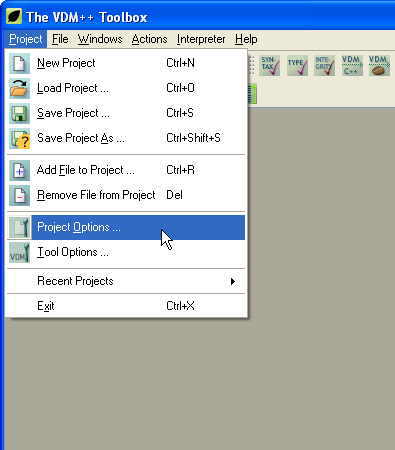
\includegraphics[width=.8\textwidth]{optionsmenu}
\caption{Selecting Java Code Generator Options}\label{fig:optionsmenu}
\end{center}
\end{figure}

The various options available in \tcg\ are shown in
Figure~\ref{fig:options}. 
\begin{figure}
\begin{center}
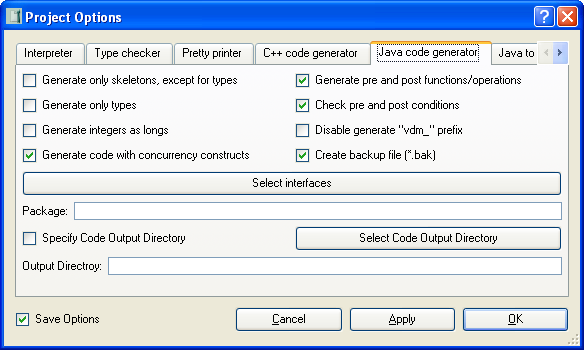
\includegraphics[width=.8\textwidth]{options}
\caption{Options for Java Code Generation}\label{fig:options}
\end{center}
\end{figure}
Each of these options is described below. Note that all of these
options are also available in the command-line version of \tcg. The
appropriate flags are shown in brackets after the name of each option
below. Default behaviour is also described with ``off'' meaning that
by default the behaviour specified by the given option is not used,
and ``on'' meaning such behaviour is used.

\begin{description}
\item [Code generate only skeletons, except for types ({\tt -s})] 
  Specify this  option to
  generate skeleton classes. A skeleton class is a 
  class containing full type, value and instance variable definitions,
  but empty function and operation definitions.  Default: \textbf{off}
%\item [Code generate small types] 
%  The default behaviour of the Code Generator is to
%  generate code with ``big'' types, i.e.\ the wrapper classes {\tt
%  Integer}, {\tt Double}, {\tt Boolean} and {\tt Character} are used
%  in the generated code. Specify the {\tt -m} option in order to
%  generate code using the ``small'' types   {\tt int}, {\tt double},
%  {\tt boolean} and {\tt char}. Note, that ``small'' types are only
%  used in type definitions and method headers. Therfore, this option
%  implies the {\tt -s} option, because otherwise the generated code
%  would not be compilable. It is not possible to insert primitive
%  data types in compound data types such as sets and sequences. %{\tt -m}
\item [Code generate only types ({\tt -u})] 
  Specify this
  option to only want to generate Java code for VDM++ type
  definitions (i.e. functions, operations, instance variables and
  values will not be generated). Default: \textbf{off}.%
\item [Code generate integers as Longs (\texttt{-L})]
  Using this
  option, it is possible to generate VDM++ integer values and
  variables as Java \texttt{Long}s instead of
  \texttt{Integer}s. Default: \textbf{off}.
\item [Code generate code with concurrency constructs (\texttt{-e})]
  This option is used to force the Code Generator to generate code
  which includes support for concurrency. See Section~\ref{concmain}
  for details of this. Default: \textbf{on}.
\item [Code generate pre and post functions/operations (\texttt{-k})] 
  Specify this option
  in order to code generate Java methods for pre and post conditions
  and invariants them. Default: \textbf{on}%{\tt -k}
\item [Check pre and post conditions (\texttt{-P})] 
  Specify this option to generate inline checks of function pre and post
  conditions, and operation pre conditions. Raise an exception if a
  check fails. This implies the
  previous option as pre and post conditions must be generated for
  compilable code to be generated. Default: \textbf{off}.%{\tt -P}
\item [Package (\texttt{-z}) \textit{packagename}] 
  The default behaviour of the code
  generator is to write the generated Java files in the directory,
  where your project file lies, or if no project file exists, in the
  directory, where the \ToolboxName\ was started. The files are part
  of an unnamed default package. Specify this
  option in order to generate a specific package
  which will contain the generated Java classes. The Code Generator
  will make a new directory using the given package name containing the
  created files and the generated files will include the appropriate
  \texttt{package} statement.%{\tt -z package\_name}
\item [Select Interfaces (\texttt{-U})]
  Select classes to be generated as Java interfaces. See
  Section~\ref{sec:interfaces} for details.
\end{description}

When starting the \ToolboxName\ from the command line the following
command has to be used:  

\begin{quote}
\begin{verbatim}
vppde -j [options] specfile(s)
\end{verbatim}
\end{quote}


\subsection{Implementing Implicit and Preliminary Functions/Operations}\label{implicit}

Implicit functions/operations and preliminary functions/operations
(specified by ``{\tt is not yet specified}'') are handled in the same
way by \tcg{}. Look at the following VDM++ class definition containing
a preliminary operation definition.

\begin{quote}
\begin{verbatim}
class A
operations
op:() ==> int
op() == is not yet specified;
end A
\end{verbatim}
\end{quote}

This class will be generated as follows:

\begin{quote}
\begin{verbatim}
public class A {
  protected external_A child = new external_A(this);
  private Integer op () throws CGException{
    return child.impl_op();
  }
};
\end{verbatim}
\end{quote}

As can be seen from the code listed above, the class \texttt{A}A contains a
protected instance variable {\tt child} of type {\tt external\_A}.
This is the case for all classes containing implicit
functions/operations or preliminary functions/operations (specified by
``{\tt is not yet specified}''). Though a class may have several of
these definitions, there will only exist one instance of this external
class. 

The method \path+op+ will call a method called \path+impl_op+ on this
instance.\footnote{{\tt impl} stands for ``to be implemented in
Java''.} The result of the \path+impl_op+ method is returned as
the result of the \path+op+ method. 

It is then the user's responsibility to implement the method
\path+impl_op+ in class {\tt external\_A}.  The input and output
parameters of the method \path+impl_op+ must be the same as those of
the method \path+op+. 

If a VDM++ class contains more than one implicit function/operation or
preliminary function/operation (specified by ``{\tt is not yet
specified}''), all methods have to be implemented in class
\path+external_<CLASSNAME>+. 

In order to make it easy for the user to implement the external class
file, \tcg\ generates a file \texttt{external\_A.java} for it.  With
the help of this  file, the generated Java code will be
compilable. However, a run-time error will occur, when a preliminary
function is called. The file {\tt external\_A.java} containing the
{\tt external\_A} class is listed below.  

\begin{quote}
\begin{verbatim}
public class external_A {
  A parent = null;
  public external_A (A parentA) {
    parent = parentA;
  }
  public Integer impl_op () throws CGException{
    UTIL.RunTime("Preliminary Operation op has been called");
    return new Integer(0);
  }
};
\end{verbatim}
\end{quote}

The easiest way to implement the {\tt external\_A} class is to 
modify the template class, i.e. the user just has to replace the code

\begin{quote}
\begin{verbatim}
UTIL.RunTime("Preliminary Operation op has been called");
return new Integer(0);
\end{verbatim}
\end{quote}

with user-defined code, in the usual way in which user-defined code
can replace generated code. (See Section~\ref{substituting} for
details.)

%Once the user has tailored the {\tt external\_<ClassName>.java} file,
%it has to be insured, that a new code generation does not overwrite
%it with a new file. Therefore, when an {\tt
%external\_<ClassName>.java} already exists, an {\tt
%external\_<ClassName>.java.default} file is generated instead. 

Note, that the generated constructor for the external class takes an
instance of the class {\tt A} as input parameter and assigns it to the
variable {\tt parent}. In this way, the implementation of preliminary
operation definitions can access the public state of the class {\tt A}.
Java methods for preliminary functions also use this constructor,
though they are not allowed to act on the internal state of a
class. They can however call an operation and thereby act on the
internal state indirectly.  

Implicitly defined functions and operations are handled in the same way as 
preliminary function and operation specifications containing the
clause ``{\tt is not yet specified}''. 

Note, that the external class can contain implicit and preliminary
operation and function definitions. In the generated template, they
can be distinguished by the generated runtime error message: 

\begin{quote}
\begin{verbatim}
UTIL.RunTime("Preliminary Operation op has been called");
\end{verbatim}
\end{quote}

for a preliminary operation definition called {\tt op} and

\begin{quote}
\begin{verbatim}
UTIL.RunTime("Implicit Function f has been called");
\end{verbatim}
\end{quote}

for an implicit function definition called {\tt f}, for example.

\subsection{Generation of Abstract Classes}

A VDM++ class is abstract if it contains preliminary function or
operation definitions, or if it is a subclass of an abstract class,
and does not provide implementations for the abstract functions and
operations that have been inherited. Thus being abstract is an
indirect property of a VDM++ class. 

In contrast, Java provides a primitive notion of abstract
classes. Thus when generating Java code, those VDM++ classes that are
identified as being abstract, will be generated as abstract Java
classes. For example, consider the VDM++ classes \texttt{A},
\texttt{B} and \texttt{C} below:

\begin{quote}
\begin{verbatim}
class A

instance variables
  protected m : nat := 1

operations
  public op : nat ==> nat
  op(n) == is subclass responsibility;

functions
  public f : int -> int
  f(i) == is subclass responsibility

end A

class B is subclass of A

operations
  public op : nat ==> nat
  op(n) ==
    return m + n

end B

class C is subclass of B

functions
  public f : int -> int
  f(i) == i + 1

end C
\end{verbatim}
\end{quote}
Class \texttt{A} contains preliminary functions and operations and is
therefore abstract. It would therefore be code generated as:
\begin{quote}
\begin{verbatim}
public abstract class A {
 
  protected Integer m = null;
  public abstract Integer op (final Integer n) throws CGException;
  public abstract Integer f (final Integer i) throws CGException;
 
} 
\end{verbatim}
\end{quote}
Class \texttt{B} inherits from abstract class \texttt{A}, and does not
provide an implementation of the function \texttt{f}. Therefore it is
also abstract:

\begin{quote}
\begin{verbatim}
public abstract class B extends A {

  public Integer op (final Integer n) throws CGException {
    return new Integer(m.intValue() + n.intValue());
  }
}
\end{verbatim}
\end{quote}

Finally, since class \texttt{C} inherits from \texttt{B} and provides
an implementation of \texttt{f}. It is therefore a normal class:
\begin{quote}
\begin{verbatim}
public class C extends B {
 
  public Integer f (final Integer i) throws CGException{
    return new Integer(i.intValue() + new Integer(1).intValue());
  }
} 
\end{verbatim}
\end{quote}


\subsection{Substituting Parts of the Generated Java Code}\label{substituting}

In a typical application, it will be necessary for the generated code
to interact with other code e.g. external libraries and/or handwritten
code. To facilitate such interaction, it is possible to modify the
generated code, in such a way that these modifications are not
overwritten if \tcg\ is rerun.

The way this is achieved is through the use of \textit{keep
tags}. These are comments in the generated Java code, which \tcg\ uses
to decide whether a portion of the code should be overwritten or not.

For example, consider the following example:
\begin{quote}
\begin{verbatim}
class Date

types
  public Day = <Mon> | <Tue> | <Wed> | <Thu> | <Fri> | <Sat> | <Sun>;
  public Month = <Jan> | <Feb> | <Mar> | <Apr> | <May> | <Jun> 
        | <Jul> | <Aug> | <Sep> | <Oct> | <Nov> | <Dec>;
  public Year = nat

instance variables
  d : Day;
  m : Month;
  y : Year

operations

  public SetDate : Day * Month * Year ==> ()
  SetDate(nd,nm,ny) ==
  ( d := nd;
    m := nm;
    y := ny );

  public today : () ==> Date
  today() ==
    return new Date()
end Date
\end{verbatim}
\end{quote}
Since neither VDM++ nor \ToolboxName\ has a primitive notion of time,
it is not possible to give a complete specification of
\texttt{today}. In the generated code, \texttt{today} is generated as
follows: 
\begin{quote}
\begin{verbatim}
// ***** VDMTOOLS START Name=today KEEP=NO
  public Date today () throws CGException{
    return (Date) new Date();
  }
// ***** VDMTOOLS END Name=today
\end{verbatim}
\end{quote}
The comments above and below the function definition represent the keep
tag for this function. In a keep tag the following information is found:
\begin{itemize}
\item The name of the entity to which the tag applies (what constitutes
an entity is explained below). This appears immediately after the text
\texttt{Name=}. 
\item A flag indicating whether this entity should be retained or
overwritten. This is given by the text after \texttt{KEEP=}. If it is
\texttt{NO}, the entity will be overwritten; if \texttt{YES} it is
retained. The default when a file is generated is \texttt{NO}.
\end{itemize}
Suppose we wish to modify this function to actually return the current
day. This is possible using the \texttt{Calendar} class provided as
part of the Java Development Kit. 
\begin{quote}
\begin{verbatim}
// ***** VDMTOOLS START Name=today KEEP=YES
  public Date today () throws CGException{
    Calendar c = Calendar.getInstance();
    Date result = new Date();
    Object td = new Object(), tm = new Object();
    switch (c.get(Calendar.DAY_OF_WEEK)){
    case Calendar.MONDAY:
        td = new quotes.Mon();
        break;
    ...
    }
    switch (c.get(Calendar.MONTH)){
    case Calendar.JANUARY:
        tm = new quotes.Jan();
        break;
    ...
    }
    result.SetDate(td, tm, new Integer(c.get(Calendar.YEAR)));
    return result;
  }
// ***** VDMTOOLS END Name=today
\end{verbatim}
\end{quote}
First note that the keep tag has been changed to \texttt{YES}. This
ensures that the changes made are preserved. The body of the function
is then normal Java code, which is able to use arbitrary external
classes. 

In addition to changing existing entities, new entities can be added
to the Java file. Suppose we wish to replace the default
\texttt{toString} method (inherited from \texttt{java.lang.Object})
with one tailored to dates. We could add the following to the class
definition. 
\begin{quote}
\begin{verbatim}
// ***** VDMTOOLS START Name=toString KEEP=YES
  public String toString(){
      return d.toString() + m.toString() + y.toString();
  }
// ***** VDMTOOLS END Name=toString
\end{verbatim}
\end{quote}

\subsubsection{Entities}

An entity is a region in a generated Java file which can be retained
using keep tags. It may be one of the following:
\begin{itemize}
\item A top-level class member variable.
\item A top-level class method (including constructors).
\item An inner class.
\item A collection of import declarations.
\item A package declaration.
\item A header comment i.e. a region at the head of the file, in which
comments can be placed, for instance version control information. 
\end{itemize}
Note that keep tags may also be used with classes generated as
interfaces (see Section~\ref{sec:interfaces}); in that case the same
rules apply, where interface should be read instead of class.

Three tag names are predefined and always appear in the generated
file: \texttt{HeaderComment} for header comments, \texttt{package} for
package declarations and \texttt{imports} for import declarations. 

\subsubsection{Rules for keep tags}

The following rules must be followed when using keep tags. 
\begin{itemize}
\item Each tag name must be unique.
\item Keep tags must be flat i.e tags can not be nested.
\item Outside a class definition, the only tags that may appear are
\texttt{HeaderComment}, \texttt{package} and \texttt{imports}. 
\item Added entities must appear \textbf{within} the class
definition, but at the top-level. Thus for instance if a function is
added to an inner class, the whole inner class must be tagged
\texttt{YES}. 
\item The syntax of keep tags is case and white-space sensitive. It
must be followed exactly.
\end{itemize}
Failure to follow these rules could lead to code being
overwritten. However since the original file is always backed up, this
need not be fatal. 


\subsection{Generating Interfaces}\label{sec:interfaces}

\Tcg\ allows generation of Java interfaces \cite{Gosling&00}. A \VDM\
class may be generated as an interface if the following conditions
apply:
\begin{itemize}
\item All of the functions and operations defined in the class have
body \texttt{is subclass responsibility}.
\item The class contains no instance variables are defined in the
class. 
\item All types defined in the class are public.
\item All values defined in the class can be defined directly (see
Section~\ref{values} for an explanation of what is meant by directly
defined values).
\item All superclasses of this class can be generated as interfaces.
\end{itemize}
For instance, consider the example in Figure~\ref{fig:interfacesex}.
\begin{figure}
\begin{quote}
\verbatiminput{manexamples/interfaces.vpp}
\end{quote}
\caption{Interfaces Example}\label{fig:interfacesex}
\end{figure}
The class \texttt{A} clearly fulfils the requirements for being
generated as an interface, since it has a directly defined value and
all of its functions and operations are \texttt{is subclass
responsibility}. Class \texttt{B} can also be generated as an
interface, since it provides just one abstract function, and inherits
from a class that can be generated as an interface. Class \texttt{C}
however can not be generated as an interface, since it declares a
non-abstract function.

To select which classes are to be generated as interfaces, click on
the \textit{Select Interfaces} button in the options dialogue box (as
described in Section~\ref{options}). A new dialogue box opens, as
shown in Figure~\ref{fig:interfaces1}.

\begin{figure}
\begin{center}
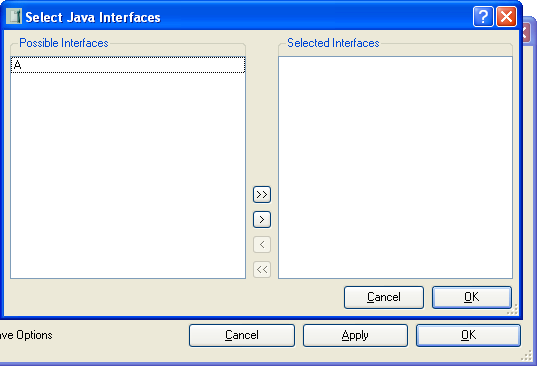
\includegraphics[width=.8\textwidth]{interfaces1}
\end{center}
\caption{Initial Interface Selection Dialogue}\label{fig:interfaces1}
\end{figure}

Initially, only one class may be generated as an interface -
\texttt{A}. If this is selected (by clicking on the \textit{Add}
button), the dialogue is updated as shown in Figure~\ref{fig:interfaces2}.

\begin{figure}
\begin{center}
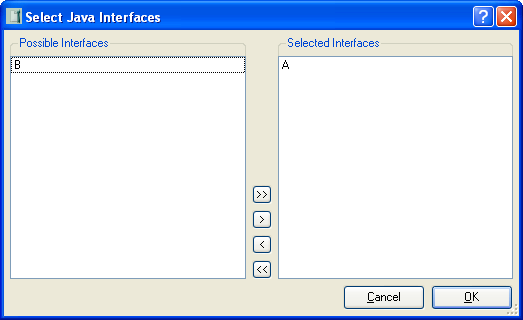
\includegraphics[width=.8\textwidth]{interfaces2}
\end{center}
\caption{Updated Interface Selection Dialogue}\label{fig:interfaces2}
\end{figure}

Note that since \texttt{B} now appears in the list of possible
interfaces. This is because it can only be generated as an interface
if its superclass - \texttt{A} - is an interface. If \texttt{A} is now
removed from the list of select interfaces, \texttt{B} will
automatically be removed from the list, since it no longer satisfies
the criteria to be an interface.

Having selected classes to be generated as interfaces, code generation
proceeds as normal. The following code would be generated for
\texttt{A}:
\begin{quote}
\begin{verbatim}
public interface A {
 
// ***** VDMTOOLS START Name=v KEEP=NO
  public static final Number v = new Integer(1);
// ***** VDMTOOLS END Name=v


// ***** VDMTOOLS START Name=op#1|Number KEEP=NO
  abstract public Number op (final Number n) throws CGException ;
// ***** VDMTOOLS END Name=op#1|Number


// ***** VDMTOOLS START Name=f#1|Number KEEP=NO
  abstract public Number f (final Number n) throws CGException ;
// ***** VDMTOOLS END Name=f#1|Number

} 
\end{verbatim}
\end{quote}

Interfaces may also be selected using the command-line version of the
Toolbox, using the \texttt{-U} option:
\begin{quote}
\begin{alltt}
vppde -j -U \textit{class\{,class\}} specfiles
\end{alltt}
\end{quote}
If a class, which does not satisfy the above interface critera, is
selected as an interface, the following error message will be
generated:
\begin{quote}
\begin{alltt}
Can not generate class \textit{class} as an interface - ignored
\end{alltt}
\end{quote}



\subsection{Limitations}\label{sec:unsupported}

Not all \VDM\ specifications can be code generated to Java. The \VDM\
specifications have to meet certain requirements in order to be
translated to compilable and correct Java code. These limitations are
caused mainly by two reasons: 
\begin{itemize}
\item Limitation of the translation algorithm used: \VDM\ and Java are
  two different languages. In a small number of 
  cases the translation of some \VDM\ constructs can lead to incorrect
  Java code. The limitations caused by this fact are listed in
  Section~\ref{lim1}. \VDM\ specifications, that does not fulfil the
  listed requirements, can result in non-compilable and incorrect Java code.
  \Tcg\ generates a warning/error message when it encounters a \VDM\
  feature not translatable to Java. 
\item Limitation of the domain of the translation: The Code Generator
  does not support all \VDM\ 
  constructs. Section~\ref{lim2} summarizes the \VDM\ constructs not
  supported by \tcg{}. These 
  constructs do not result in uncompilable Java code, but the
  execution of the generated code for these constructs will result in
  run-time errors.  \Tcg\ will give a warning whenever an unsupported
  construct is encountered.
\end{itemize}
Note that the semantics of Java and VDM++ differ with respect to how
private methods are handled with respect to dynamic dispatch. Consider
the following example:

\begin{minipage}{.55\textwidth}
\begin{quote}
\begin{verbatim}
class C
operations
public op1 : () ==> seq of char
op1() == op2();

private op2 : () ==> seq of char
op2() == return "C`op2"
end C
\end{verbatim}
\end{quote}
\end{minipage}
\begin{minipage}{.45\textwidth}
%\begin{quote}
\begin{verbatim}
class D is subclass of C
operations
public op3 : () ==> seq of char
op3() == op1();

private op2 : () ==> seq of char
op2() == return "D`op2"
end D
\end{verbatim}
%\end{quote}
\end{minipage}

In Java, the expression \texttt{new D().op3()} yields the result
\texttt{C`op2}. In \VDM\ the same expression yields \texttt{"D`op2"}. 

\subsubsection{Requirements of \VDM\ specifications due to language differences}
\label{lim1}

The \VDM\ specification has to meet the following requirements in
order to generate {\em compilable} and {\em correct} Java code:

\begin{itemize}
\item Type checker warnings as ``{\em Missing type information}'' should
  be removed, because they can lead to errors in the generated code.
  \Tcg\ is not able to generate correct Java types, if type information is
  missing for a VDM construct.

\item Classes, instance variables, types, values, functions and operations may not have the same name.
%Moreover, redeclaration of names should be avoided. That means, the following \VDM\ specification for
%example will result in non-compilable code because the variable name {\tt a} is redeclared:
%
%\begin{quote}
%\begin{small}
%\begin{verbatim}
%f : int | (int * int) ==> bool
%f(a) ==
%  cases a:
%    2 -> return true,
%    mk_(a,b) ->  return false,
%    others -> let a = 1 in return true
%  end;
%\end{verbatim}
%\end{small}
%\end{quote}

\item Abstract operations/functions must have the same type as the
operations/functions implementing them. Consider the following example: 
\begin{quote}
\begin{small}
\begin{verbatim}
class A
operations
  m: nat ==> nat
  m(n) == is not yet specified;
end A

class B is subclass of A
operations
  m: nat ==> nat
  m(n) = return n+n;
end B
\end{verbatim}
\end{small}
\end{quote}
If the type of \texttt{B`m} did not exactly match that of
\texttt{A`m}, then \texttt{A`m} would still be abstract in \texttt{B},
and therefore \texttt{B} would be an abstract class.

\item A limited form for multiple inheritance may be used. However,
the classes involved have to fulfil the conditions described in
Section~\ref{sec:interfaces}.

\item If all branches in a case statement contain a return statement,
the case statement must have an {\tt others} branch.
Otherwise the Java compiler generates a  ``{\em Return required}'' error when compiling the generated Java code.

\item Dead code should be avoided. Consider the following example:

\begin{quote}
\begin{small}
\begin{verbatim}
operations
  m : nat ==> nat
  m(n) ==
    (return n;
     a:= 4;
    );
\end{verbatim}
\end{small}
\end{quote}

The statement {\tt a:= 4;} will never be executed, which leads to an ``{\em Statement not reached}''
error when compiling the generated Java code.

\item When operation calls in a superclass are qualified by name, the generated code can be erroneous.
Look at the following example:

\begin{quote}
\begin{small}
\begin{verbatim}
class A

operations

public SetVal : nat ==> ()
SetVal(n) == ...;

end A

class B is subclass of A

operations

public SetVal : nat ==> ()
SetVal(n) == ...

end B

class C is subclass of B

operations

public Test : () ==> ()
Test() ==
  ( self.SetVal(1);
    self.B`SetVal(1);
    self.A`SetVal(2)
  )

end C

class D

instance variables
  b : B := new B()

operations

public Test: () ==> ()
Test() ==
  (b.SetVal(1);
   b.B`SetVal(5);
   b.A`SetVal(2)
  )

end D
\end{verbatim}
\end{small}
\end{quote}

  Let us start looking at class {\tt C}: The statement {\tt self.SetVal(1)}
  calls the {\tt SetVal} operation in class {\tt C} and will be code generated
  as {\tt this.SetVal(1)} in Java.  The statement {\tt self.B`SetVal(1)}
  calls the {\tt SetVal} operation in class  {\tt B} and will be code generated
  as {\tt super.SetVal(1)} in Java.  In Java it is impossible to
  call the {\tt SetVal()} method in class {\tt A}.  The statement {\tt
    self.A`SetVal(2)} will be code generated as {\tt
    super.SetVal(2)}. If there was no {\tt SetVal} operation in
  class {\tt B}, this would be correct. However, in the above case, this is
  not in conformity with the VDM++ specification. 
  The two operation calls
  {\tt self.B`SetVal(1)} and {\tt self.A`SetVal(2)} will cause the
  Code Generator to give the warning ``{\em Quoted method call is code generated as a call to super}''.
  The user can then make sure if the correct method is called.
  
  Let us now look at class {\tt D}: The statement {\tt b.SetVal(1)} calls
  the {\tt SetVal} operation in class {\tt B} and will be code generated as
  {\tt b.SetVal(1)} in Java. In Java it is not possible to invoke
  overriden methods from outside the class that does the overriding.
  There is therefore no way to call the {\tt SetVal} method in class {\tt A}.
  The quoted operation calls in class {\tt D} are therefore all code
  generated as {\tt b.SetVal(1)}. The code generating will however
  give the warning ``{\em Quoted method call is removed}'' in order to
  inform the user.

\item The max (min) values for integer and double types in Java are
  smaller (bigger) than the respective values in \VDM{}. Values, that
  are not valid in Java lead to errors when running the generated Java
  code. 
\end{itemize}

\subsubsection{Unsupported Constructs}
\label{lim2}

In this version of \tcg\ the following \VDM\ constructs are not supported:

\begin{itemize}

%% Is not part of the language manual any longer!
%\item The Real-time part of \VDM{}. 
\item Expressions:

  \begin{itemize}
  \item Lambda.
  \item Compose, iterate and equality for functions.
  \item Type judgement expressions with type variable.
#ifdef VICEMAN
  \item Time expressions.
#endif VICEMAN
  \item Higher order functions.
  \item Local function definitions.
  \item Function type instantiation expression. However, the code
    generator supports function type instantiation expression in
    combination with apply expression, as in the following example:

\begin{quote}
\begin{verbatim}
Test:() -> set of int
Test() ==
  ElemToSet[int](-1);

ElemToSet[@elem]: @elem +> set of @elem
ElemToSet(e) ==
  {e}
\end{verbatim}
\end{quote}

  \end{itemize}

\item Statements: 

  \begin{itemize}
  \item Specification statements.
#ifdef VDMSL
  \item `{\sf using}' in call statement.
#endif VDMSL
%#ifdef VDMPP
%  \item Start list statements.
%#endif VDMPP
#ifdef VICEMAN
  \item Duration and cycle statements are ignored.
#endif VICEMAN
  \end{itemize}

\item Type binds (see \langmancite) in:

  \begin{itemize}
  \item Let-be-st expression/statements.
  \item Sequence, set and map comprehension expressions.
  \item Iota and quantified expressions.
  \end{itemize}

As an example the following expression is supported by \tcg :

\begin{quote}
\begin{verbatim}
let x in set numbers in x
\end{verbatim}
\end{quote}

whereas the following is not (caused by the type bind \verb+n: nat+):

\begin{quote}
\begin{verbatim}
let x: nat in x
\end{verbatim}
\end{quote}

\item Patterns in complex form: 

  \begin{itemize}
  \item Set union pattern.
  \item Sequence concatenation pattern.
  \item Map munion pattern.
  \end{itemize}

#ifdef VDMSL
\item Local Function Definitions.

\item Higher order function definitions.
  
\item Function Values. 

\item Parameterized modules.
#endif VDMSL
\end{itemize}

#ifdef VICEMAN
System specifications and the corresponding deployment to CPUs and
BUSes is ignored. If Java code is generated from such system
descriptions the generated code is useless and will not be able to
compile. In the same way the \keyw{async} keyword in front of
operation definitions is ignored.
#endif VICEMAN

\Tcg\ is able to generate compilable code for
specifications including these constructs, but the execution of the
code will result in a run-time error if a branch containing an
unsupported construct is executed. Consider the following function
definition:

\begin{quote}
\begin{verbatim}
f: nat -> nat
f(x) ==
  if x <> 2 then
    x
  else
    iota x : nat & x ** 2 = 4
\end{verbatim}
\end{quote}

The code generated for \path+f+ will be compiled.  The
compiled Java code corresponding to \path+f+ however will result in a run-time
error if \path+f+ is applied with the value 2, as type binds in iota
expression are not supported.

Note, that \Tcg\ will give a warning whenever an unsupported construct
is encountered. Generating code for the function {\tt f} listed above
leads to the {\em Error} window shown in Figure~\ref{fig:cg_error}.

\begin{figure}[H]
\begin{center}
\mbox{}
\resizebox{9.2cm}{!}{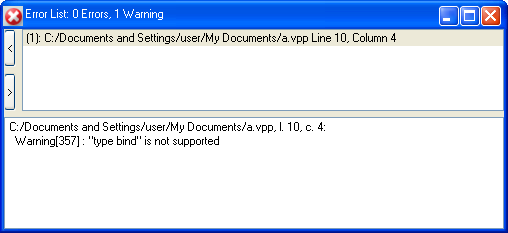
\includegraphics{warning}}
\caption{A warning generated by the Code Generator.}\label{fig:cg_error}
\end{center}
\end{figure}

\newpage
\section{Code Generating \VDM\ Specifications}
\label{sec:relation}

This section will give you a detailed description of the way \VDM\
constructs are code generated, including classes, types, values,
instance variables, functions, operations, expressions and statements.
This description should be studied intensively by those wishing to use
\tcg\  professionally. 

We will start by giving an introduction to the \JL{}, which forms the
basis of code generating \VDM\ specifications.
Afterwards, we will describe the code generated for the above mentioned
\VDM\ constructs, one by one.

\subsection{The VDM Java Library}
\label{VDMlib}

The data refinement of the generated code is based on the \JL{}, which
is implemented in the package {\tt jp.vdmtools.VDM}. Here, we will
only give a short introduction to this library. It is further described by
HTML documentation generated by the {\em javadoc} program. In order to
get a full understanding of this library you should read that
documentation. See Appendix~\ref{install} for a description about how
to generate the HTML documentation using the {\em javadoc} program.

The \JL{} provides a fixed implementation of the following
\VDM\ data types: 

\begin{itemize} 
%\item Sequence Type
%\item Set Type
%\item Map Type
%\item Quote Type
%\item Token Type
\item Product/Tuple Type
%\item Optional Type
\item Record Type
\end{itemize}

For each of these types a class has been implemented providing the
same public methods as the corresponding VDM++ type. These classes 
are implemented on top of classes provided by the Java language. 

\VDM\ data types, which are not listed above (the basic \VDM\ 
data types, sets, sequences, maps, the \path+Optional+ type and the
\path+Object Reference+ 
type) are represented by classes/constructs which are part of the Java
language itself, or part of the standard Java Development Kit (JDK)
distribution. 

In addition to providing an implementation of the above listed \VDM\
data types, the \JL{} provides two more classes: 

\begin{itemize}
\item The {\tt UTIL} class.

This class contains auxiliary methods, which are used in the generated code and
which can be used by the user when interfacing the generated code.
The most important of these auxiliary methods are listed below:
\begin{itemize}
\item {\tt clone}: clones (in-depth) a VDM value. However,
  \VDM\ classes and basic \VDM\ data types are not cloneable.
\item {\tt equals}: compares two VDM values.
\item {\tt toString}: returns a String containing an ASCII representation of a VDM value.
\item {\tt RunTime}: is called when a run-time error occurs. It throws
  a {\tt VDMRunTimeException}, which is defined in the \JL{}.
\item {\tt NotSupported}: is called when an unsupported construct is executed. 
It throws a {\tt NotSupportedConstructException}, which is defined in the \JL{}.
\end{itemize}

Note: Use always the {\tt clone}, {\tt toString} and {\tt equals} methods of the {\tt UTIL} class - and
not the methods defined in the Java classes corresponding to VDM++ data types.

\item The {\tt CGException} class and its subclasses.
  
The error handling of the VDM Java library is based on Java's exception
handling mechanism.  When an error is detected by the generated Java
code or one of the library methods, an appropriate exception is
thrown.  All the implemented errors are subclasses of the class {\tt
CGException}, which again is a subclass of the {\tt java.lang.Exception} class.  
The inheritance structure of the exception classes is shown in
Figure~\ref{fig:exceptionclasses}. 

\begin{figure}[tbh]
\begin{center}
\mbox{}
\begin{picture}(400,250)
\put(0,0){\framebox(180,50){VDMLibRunTimeException}}
\put(220,0){\framebox(180,50){NotSupportedConstructException}}
\put(110,100){\framebox(180,50){CGException}}
\put(110,200){\framebox(180,50){Exception}}

\put(90,50){\line(0,1){25}}
\put(310,50){\line(0,1){25}}
\put(90,75){\line(1,0){220}}
\put(200,75){\line(0,1){25}}
\put(200,150){\line(0,1){50}}

\end{picture}
\caption{Inheritance structure of the Java classes handling Code Generator exceptions.\label{fig:exceptionclasses}}
\end{center}
\end{figure}

The different kinds of exceptions are grouped into two types.
\begin{itemize}

\item Instances of the {\tt VDMRunTimeException} class: They are
thrown in the generated Java code. They correspond to run-time errors
occuring when executing \VDM\ specifications.  

\item Instances of the {\tt NotSupportedConstructException} class:
They are thrown when constructs not supported by \tcg\ are executed.  

\end{itemize}
\end{itemize}

\subsection{Code Generating Classes}
\label{sec:classes}

For each \VDM\ class a corresponding Java class is generated. For each
\VDM\ class member, the corresponding item in the  Java class will
have the same access modifier as the \VDM\ member.

Let us have a closer look at the structure of a Java class generated
for a class in the \VDM\ specification. 

The generated Java class contains:

\begin{itemize}
%\item A static \textit{comparator}, implementing the interface
%\texttt{java.util.Comparator} in the Java Development Kit. This is
%used in tree-based data structures, and implements the VDM notion of equality. 
\item Java code implementing \VDM\ datatypes. (See Section~\ref{types})
\item Java code implementing \VDM\ values. (See Section~\ref{values})
\item Java code implementing \VDM\ instance variables. (See Section~\ref{sec:instvars})
\item A static initializer (if values have to be initialized).
\item A instance variable initializer (called from constructor).
\item A constructor (if the class contains instance variable definitions).
\item Java methods implementing \VDM\ functions. (See Section~\ref{funcop})
\item Java methods implementing \VDM\ operations. (See Section~\ref{funcop})
#ifdef VDMPP
\item Code for concurrency (synchronization, threads etc), if that
option is selected; see Section~\ref{concmain}.
#endif VDMPP
\end{itemize}

Consider the resulting skeleton of a generated Java class, generated
for a \VDM\ class definition, say {\tt A}: 

\begin{quote}
\begin{verbatim}
public class A {

// ***** VDMTOOLS START Name=vdmComp KEEP=NO
  static UTIL.VDMCompare vdmComp = new UTIL.VDMCompare();
// ***** VDMTOOLS END Name=vdmComp

  ...Implementation of VDM++ types...
  ...Implementation of VDM++ values... 
  ...Implementation of VDM++ instance variables... 

// ***** VDMTOOLS START Name=static KEEP=NO
  static {
         ...Initialization of VDM++ values...
         }
// ***** VDMTOOLS END Name=static

// ***** VDMTOOLS START Name=A KEEP=NO
  public A () { 
      try { ...
            Initialization of VDM++ instance variables...
            ...
          }
      catch (Throwable e) { ...
                          }
  }
// ***** VDMTOOLS END Name=A

  ...Implementation of VDM++ functions... 
  ...Implementation of VDM++ operations... 

};
\end{verbatim}
\end{quote}

If a \VDM\ class is abstract, the generated Java class
will also be declared as such. 

\subsection{Inheritance Structure of the Generated Java Classes}
\label{inheritance}
The inheritance structure of the generated Java classes corresponds
exactly to the inheritance structure of the \VDM\ classes. 

The inheritance structure of the \VDM\ classes and the generated Java
classes for the sorting example is shown in Figure~\ref{fig:sortppjava}.

\begin{figure}[H]
\begin{center}
\subfloat[VDM++]{
\begin{picture}(200,125)
\put(0,0){\framebox(50,50){
  \parbox{1.75cm}{\centering
  Merge Sort}
}
}
\put(60,0){\framebox(50,50){
  \parbox{1.75cm}{\centering
  ExplSort}
}}
\put(120,0){\framebox(50,50){
  \parbox{1.75cm}{\centering
  ImplSort}
}}
\put(180,0){\framebox(50,50){
  \parbox{1.75cm}{\centering
  DoSort}
}}
\put(90,75){\framebox(50,50){Sorter}}
\put(25,62){\line(1,0){180}}
\put(25,50){\line(0,1){12}}
\put(85,50){\line(0,1){12}}
\put(145,50){\line(0,1){12}}
\put(205,50){\line(0,1){12}}
\put(115,62){\line(0,1){13}}
\end{picture}
}\quad
\subfloat[Java]{
\begin{picture}(200,200)
\put(0,0){\framebox(50,50){
  \parbox{1.75cm}{\centering
  Merge Sort}
}
}
\put(60,0){\framebox(50,50){
  \parbox{1.75cm}{\centering
  ExplSort}
}}
\put(120,0){\framebox(50,50){
  \parbox{1.75cm}{\centering
  ImplSort}
}}
\put(180,0){\framebox(50,50){
  \parbox{1.75cm}{\centering
  DoSort}
}}
\put(90,75){\framebox(50,50){Sorter}}
\put(90,150){\framebox(50,50){Object}}
\put(25,62){\line(1,0){180}}
\put(25,50){\line(0,1){12}}
\put(85,50){\line(0,1){12}}
\put(145,50){\line(0,1){12}}
\put(205,50){\line(0,1){12}}
\put(115,62){\line(0,1){13}}
\put(115,125){\line(0,1){25}}
\end{picture}
}
\end{center}
\caption{Inheritance structure of the VDM++ classes and the generated Java classes}\label{fig:sortppjava}

\end{figure}

\VDM\ allows classes to have more than one superclass, using multiple
inheritance. Java does not support multiple inheritance. Instead,
Java replaces multiple inheritance with interfaces \cite{Gosling&00}.
A class in Java optionally {\tt extends} one superclass and it
optionally {\tt implements} one or more interfaces. In order to
implement an interface, a class must first declare the interface in an
{\tt implements} clause, and then it must provide an implementation for
all the abstract methods of the interface. This is actually the real
difference between multiple inheritance in \VDM\ and interfaces in
Java. In Java, a class can inherit actual implementations only from
one superclass. It can inherit additional {\tt abstract} methods from
interfaces, but it must provide its own implementation of these
methods.

To resolve multiple inheritance at the VDM++ level, the user must
select which classes are to be code generated as interfaces (see
Section~\ref{sec:interfaces} for details of how this is done).
Since Java's interface model is more simple than the \VDM\ multiple
inheritance model, not all cases of multiple inheritance in \VDM\ can
be suitable resolved. In such circumstances the \VDM\ model must be
modified if complete code generation is desired. 

In order to generate Java
code for multiple inheritance in \VDM{} the superclasses in \VDM\ 
must fulfil the following conditions:

\begin{itemize}
\item Only one superclass may define functions and operation
  implementations, and only this superclass may provide instance
  variables. This class will be code generated as the single
  superclass in Java. 
\item It must be possible to generate all other superclasses as
  interfaces (see Section~\ref{sec:interfaces}).
\end{itemize}
Note that if the subclass does not provide implementations for all
abstract functions and operations that are inherited, it will be
generated as an abstract class.

Consider the following example of a \VDM\ specification, that can be
code generated: 

\begin{quote}
\begin{small}
\begin{verbatim}
class E

instance variables
  protected i : nat

end E

class F

values
  public n : nat = 3

operations
  public  getx : () ==> nat
  getx() == is subclass responsibility;

end F

class G is subclass of E, F

operations
  public  getx : () ==> nat
  getx() == if true then return n else return i;

end G
\end{verbatim}
\end{small}
\end{quote}

The listed \VDM\ specification fulfils the necessary conditions:
Class {\tt G} is the subclass of the two classes {\tt E} and {\tt F}.
Class {\tt E} defines an instance variable. Therefore it will be code
generated as the single superclass in Java. Class {\tt F} may be
generated as an interface, since it fulfils the criteria given in
Section~\ref{sec:interfaces}. 

The generated Java code for \texttt{G} is listed below.

\begin{quote}
\begin{small}
\begin{verbatim}
public class G extends E implements F {

// ***** VDMTOOLS START Name=vdm_init_G KEEP=NO
  private void vdm_init_G () {}
// ***** VDMTOOLS END Name=vdm_init_G


// ***** VDMTOOLS START Name=G KEEP=NO
  public G () throws CGException {
    vdm_init_G();
  }
// ***** VDMTOOLS END Name=G


// ***** VDMTOOLS START Name=getx KEEP=NO
  public Number getx () throws CGException {
    if (true)
      return n;
    else
      return i;
  }
// ***** VDMTOOLS END Name=getx

}
;
\end{verbatim}
\end{small}
\end{quote}

If the \VDM\ specification does not fulfil the above listed
requirements, the \cg\ will generate incorrect code.

If multiple inheritance at the \VDM\ level is not resolved, \tcg\
will result in the following error: 
\begin{verbatim}
Error : "Multiple inheritance in this form" is not supported and is not 
        code generated
\end{verbatim}

Note: The VDM++ expressions {\em Base Class}, {\em Class}, {\em Same
Base Class} and {\em Same Class} Membership will have a different
semantics for generated Java code compared to the original \VDM\
specification, in the presence of multiple inheritance.

\subsection{Code Generating Types}
\label{types}
 In this section the way \VDM\ types are mapped into Java code is described. 
In addition, the naming conventions for types are summarized.


\subsubsection{Mapping Anonymous \VDM\ Types to Java}

Anonymous types are types that are not given a name in the \VDM\
specification. The way in which they are code generated is described
in the following sections.

\paragraph{The Boolean, Numeric and Character Types}
  
  The Java language package provides the following ``wrapper'' classes
  for the primitive data types double, int, boolean and char: {\tt
  Double}, {\tt Integer}, {\tt Boolean} and {\tt Character}
  respectively.  These classes are used to represent the following
  \VDM\ datatypes: 
  \path+real+, \path+ rat+, \path+int+, \path+nat+, \path+nat1+, 
  \path+bool+, \path+char+.
  The VDM \path+real+ and \path+rat+ types are mapped to the Java
  class {\tt Double}. The VDM \path+nat+, \path+nat1+ and \path+int+
  types are mapped to the Java class {\tt Integer}. The VDM
  \path+bool+ type is mapped to the Java class {\tt Boolean}. The VDM
  \path+char+ type is mapped to the Java class {\tt Character}.
  
  Note that there is a semantic difference here between \VDM\ and
  Java. In \VDM\ the \path+int+, \path+nat+, \path+nat1+ types are
  subtypes of the \path+real+ and \path+rat+ types. This means, that it is
  possible to assign an integer to a variable of type \path+real+ and
  it is possible to assign a real to a variable of type \path+int+, if
  its value is an integer value.

  In Java objects of type {\tt Double} and \path+Integer+ cannot be
  cast to each other in the same way. Therefore, two auxiliary Java 
  methods: \path+UTIL.NumberToDouble+ and
  \path+UTIL.NumberToInteger+ have been provided. The \path+Number+
  class is a superclass to both the \path+Double+ and the
  \path+Integer+ class.

\paragraph{The Quote Type}

\Tcg{} generates a class definition for every quote used in the VDM++
  specification. All quotes are collected in the \verb+quotes+
  package. The   quote \verb+<HELLO>+ will lead to the {\tt HELLO}
  class definition in file {\tt HELLO.java} in the package {\tt
  quotes}: 

\begin{quote}
\begin{small}  
\begin{verbatim}
package quotes;

public class HELLO {

  static private int hc = 0;

  public HELLO () {
    if (hc == 0) 
      hc = super.hashCode();
  }

  public int hashCode () {
    return hc;
  }

  public boolean equals (Object obj) {
    return obj instanceof HELLO;
  }

  public String toString () {
    return "<HELLO>";
  }
};
\end{verbatim}
\end{small}  
\end{quote}

The quote \verb+<HELLO>+ can then be code generated as follows:
\begin{quote}
\begin{alltt}
new quotes.HELLO()
\end{alltt}
\end{quote}
Note that the \texttt{hashCode} method ensures that every instance of
a quote constant has the same hash code.

\paragraph{The Token Type}

 \Tcg{} generates a \verb+Token+ class in the file
  \verb+Token.java+ when the VDM++ specification contains a
  token type:


\begin{quote}
\begin{small}  
\begin{verbatim}
import jp.co.csk.vdm.toolbox.VDM.*;

public class Token {

  Object vdmValue;

  public Token (Object obj) {
    vdmValue = obj;
  }
  public Object GetValue () {
    return vdmValue;
  }
  public boolean equals (Object obj) {
    if (!(obj instanceof Token)) 
      return false;
    else 
      return UTIL.equals(this.vdmValue, ((Token) obj).vdmValue);
  }
  public String toString () {
    return "mk_token(" + UTIL.toString(vdmValue) + ")";
  }
};
\end{verbatim}  
\end{small}  
\end{quote}

The token value \verb+mk_token(<HELLO>)+ is for example code generated as follows:

\begin{quote}
\begin{alltt}
new Token(new quotes.HELLO());
\end{alltt}
\end{quote}

\paragraph{The Sequence, Set and Map Types}

The VDM Sequence (except the {\tt seq of char} type), Set and Map
types are mapped to the \texttt{Vector}, \texttt{TreeSet} and
\texttt{HashMap} classes of the \texttt{java.util} package. For
\texttt{TreeSet}s, comparison is based on the comparator defined in the
\texttt{UTIL} class provided. These classes respectively implement the 
interfaces \texttt{List}, \texttt{Set} and \texttt{Map}, also
defined in the \texttt{java.util} package.

The {\tt seq of char} type is mapped into the Java language class {\tt
  String}. Note that for example the ``{\tt (seq of char | seq of
  nat)}'' and the ``{\tt seq of (char | nat)}'' types are generated as
  {\tt Vector}. 

\paragraph{The Tuple/Product Type}

The values of a product type are called tuples.
The class, which models the VDM Tuple Type, is called \path+Tuple+ and
can be found in the \JL{}.  

Note, that both the \VDM\ types, i.e. {\tt int * real} and {\tt seq of nat * nat}
are simply code generated as \path+Tuple+.

\paragraph{The Union Type}

Anonymous \VDM\ Union types are supported by the Java {\tt Object} class. 

\paragraph{The Optional Type} 
  
  The VDM Optional Type is represented by the fact that object
  references may be ``null'' in Java.

\paragraph{The Object Reference Type}
  
  In Section~\ref{sec:classes} it has been described, how a Java class
  is generated for each \VDM\ class.  In \VDM\, an object reference
  type is denoted by a class name.  The class name in the object
  reference type must be the name of a class defined in the
  specification.  Moreover, in \VDM\, a value of the object reference
  type can be regarded as a reference to an object.
  
The object reference type corresponds to Java's class/instance scheme.
Java manipulates objects ``by reference'' as is the case for \VDM{}.

\paragraph{The Function Type}

The \VDM\ Function Type is not supported in \tcg{}.


\subsubsection{Mapping \VDM\ Type Definitions to Java}

For \VDM\ record types, and union types consisting entirely of
records, \cg{} generates inner classes representing the types. For
other kinds of type definition, it is not necessary to generate a Java
representation, since all other type definitions are shallow
definitions. That is, they simply represent a new name for an existing
type. In such cases \cg{} instead uses the existing type, and the new
name is not used. To illustrate this, consider the following example:
\begin{quote}
\begin{verbatim}
types
 A = nat
 B = seq of char
 C = A | B
\end{verbatim}
\end{quote}

The new types will always be equal to
the types on the right hand side. Thus, they are just new names for
the existing types on the right hand side. Therefore, the generated code will
use the Java implementation of these right hand side types
instead. When the types {\tt A}, {\tt B} or {\tt C} are used in the
\VDM\ specification, they will be mapped to the Java classes
\path+Integer+, \path+Vector+ and \path+Object+ respectively.

However, the Record types and Union types composed of
Record types represent deep type definitions. That is, they introduce
new types to the model. Therefore they are code generated in the
manner described below: 
\begin{itemize}
\item {\em The Composite/Record Type}
    
  All record types defined in a \VDM\ specification are mapped to
  class definitions, that implement the {\tt Record} interface found
  in the \JL{}.  Fields in a record become variables in the new class.

For example, the following composite type\footnote{Note: Do not use the {\tt compose of} syntax to define composite types.}

\begin{quote}
\begin{verbatim}
public A::     real
           k : int
\end{verbatim}
\end{quote}

will be code generated as:
\begin{quote}
\begin{small}
\begin{verbatim}
public static class A implements Record {

    public Double f1;
    public Integer k;

    public A () {}
    public A (Double p1, Integer p2){
      f1 = p1;
      k = p2;
    }
    public Object clone () {
      return new A(f1,k);
    }
    public String toString () {
      "mk_G`A(" + UTIL.toString(f1) + "," + UTIL.toString(k) + ")";
    }
    public boolean equals (Object obj) {
      if (!(obj instanceof A))
        return false;
      else {
        A temp = (A) obj;
        return UTIL.equals(f1, temp.f1) && UTIL.equals(k, temp.k);
      }
    }
    public int hashCode () {
      return (f1 == null ? 0 : f1.hashCode()) + 
             (k == null ? 0 : k.hashCode());
    } 
};
\end{verbatim}
\end{small}  
\end{quote}

For each field in the record, a public instance variable has been
added to the generated class definition. The names of these variables
match the names of the corresponding VDM record field selectors.  
If a field selector is missing, the position of the element in the
record will be used instead, e.g. \verb+f1+ in the example above. If
\verb+f1+ is already used as a field selector, then the character
``f'' will be repeatedly appended until a unique field selector is obtained.

\item {\em Union Types composed of composite types}

Union types, that are composed of composite types are code generated using Java interfaces. Look at the following VDM++ types:

\begin{quote}
\begin{verbatim}
Item = MenuItem | RemoveItem;
MenuItem = Seperator | Action;
Action:: text: String;
Separator::;
RemoveItem::;
\end{verbatim}
\end{quote}

The generated Java code looks as:

\begin{quote}
\begin{small}  
\begin{verbatim}
  public static interface Item {
  };

  public static interface MenuItem extends Item {
  };

  private static class Action implements MenuItem , Record {
    ...
  } ;

  private static class Separator implements MenuItem , Record {
    ...
  } ;

  private static class RemoveItem implements Item , Record {
    ...
  } ;
\end{verbatim}
\end{small}  
\end{quote}

As you can see, the classes generated for Record types implement the interfaces generated for the Union types.
\end{itemize}

\subsubsection{Invariants }

When an invariant is used to restrict a \VDM\ type definition in the
specification, an invariant \VDM\ function is also available. This
invariant function can be called in the same scope as its associated
type definition (see \langmancite). When the option for generating pre
and post functions/operations is
chosen, the \cg{} generates a Java method definition corresponding to
such an invariant function. As an
example, consider the following \VDM{} type definition:

\begin{quote}
\begin{verbatim}
public S = set of int
inv s == s <> {}
\end{verbatim}
\end{quote}

The method declaration corresponding to the \VDM{} function {\tt
  inv\_S} is listed below.

\begin{quote}
\begin{verbatim}
public Boolean inv_S(final TreeSet s) throws CGException {
...
};
\end{verbatim}
\end{quote}

Note, that the \cg{} does not support dynamic check of invariants, but
invariant functions can be called explicitly.

\subsection{Code Generating Values}
\label{values}

\VDM\ value definitions are translated to static final variables of
the generated Java class. The static keyword is used
to indicate that a particular variable is a class variable rather than
an instance variable. Moreover, the final keyword indicates, that the variable is a constant.

Consider the example below:

\begin{quote}
\begin{verbatim}
class A
values
  public mk_(a,b) = mk_(3,6);
  private c : char = 'a';
  protected d        = a + 1;
  e        = 2 + 1;
end A
\end{verbatim}
\end{quote}

The generated class variables in the Java class {\tt A} will look like:

\begin{quote}
\begin{small}
\begin{verbatim}
public class A {
  public static final Integer a;
  public static final Integer b;
  private static final Character c = new Character('a');
  protected static final Integer d;
  private static final Integer e = new Integer(new Integer(2).intValue() + 
                                               new Integer(1).intValue());
}
\end{verbatim}
\end{small}
\end{quote}

If the \VDM\ values are initialized by a simple expression, that in
addition does not contain any other \VDM\ values, the corresponding
Java variables are initialized ``directly''. As the example shows, the
variables {\tt c} and {\tt e} are intialized directly.  The other
variables are initialized in the static initializer of the class. The
static initializer is an initialization method for class variables. It
is invoked automatically by the system when the class is loaded.  The
instance variables {\tt a}, {\tt b} and {\tt d} are thus initialized
in the static initializer of the generated Java class {\tt A}.  The static
initializer for class A is listed below:

\begin{quote}
\begin{small}
\begin{verbatim}
 static {
    Integer atemp = null;
    Integer btemp = null;
    Integer dtemp = null;    

    /** Initialization of class variables a & b */
    boolean succ_2 = true;
    {
      try{        
        Tuple tmpVal_1 = new Tuple(2);
        tmpVal_1 = new Tuple(2);
        tmpVal_1.SetField(1, new Integer(3));
        tmpVal_1.SetField(2, new Integer(6));
        succ_2 = true;
        {          
          Vector e_l_7 = new Vector();
          for (
          int i_8 = 1; i_8 <= tmpVal_1.Length(); i_8++) 
            e_l_7.add(tmpVal_1.GetField(i_8));
          if (succ_2 = 2 == e_l_7.size()) {
            atemp = UTIL.NumberToInt(e_l_7.get(0));
            btemp = UTIL.NumberToInt(e_l_7.get(2 - 1));
          }
        }
        if (!succ_2)
          UTIL.RunTime("Pattern match did not succeed in value definition");
      }
      catch (Throwable e) {
        System.out.println(e.getMessage());
      }
    }
    a = atemp;
    b = btemp;

    /** Initialization of class variable d */
    {
      try{        
        Integer tmpVal_11 = null;
        tmpVal_11 = new Integer(a.intValue() + new Integer(1).intValue());
        dtemp = tmpVal_11;
      }
      catch (Throwable e) {
        System.out.println(e.getMessage());
      }
    }
    d = dtemp;
  }
\end{verbatim}
\end{small}
\end{quote}


\subsection{Code Generating Instance Variables}
\label{sec:instvars}

The code generation of instance variables is very straightforward.
Instance variables are translated into member variables of the
corresponding Java class. 

Consider the following instance variable declaration in \VDM{}: 

\begin{quote}
\begin{verbatim}
class A
instance variables
  public i : nat;
  private k : int := 4;
  protected message : seq of char := [];
  inv len message <= 30;
  j : real := 1;
...
end A
\end{verbatim}
\end{quote}

The corresponding Java code generated by \tcg\ in file \path+A.java+ will
become:

\begin{quote}
\begin{verbatim}
public class A {
  static UTIL.VDMCompare vdmComp = new UTIL.VDMCompare();
  public Integer i = null;
  private Integer k = null;
  protected String message = null;
  private Double j = null;
  ...
}
\end{verbatim}
\end{quote}

Instance variables are initialized when an object is created.  In
Java, instance variables are initialized in the constructor
methods, which are run when an instance of the class is created.

Thus, the implementation of the constructor method for class \path+A+
initializes the instance variables as shown below:

\begin{quote}
\begin{verbatim}
public class A {
  public A () {
    try{
      k = new Integer(4);
      message = UTIL.ConvertToString(new String());
      j = UTIL.NumberToReal(new Double(1));
    }
    catch (Throwable e) {
      System.out.println(e.getMessage());
    }
  }
  ...
}
\end{verbatim}
\end{quote}

Note: Invariant definitions specified in instance variable blocks are
ignored by \tcg{}.   


\subsection{Code Generating Functions and Operations}
\label{funcop}

In \VDM{}, functions and operations can be defined both explicitly or
implicitly. The \cg{} generates Java methods for both implicit and
explicit function and operation definitions.  

In both \VDM\ and Java all functions and operations are
virtual, so there is no difference
in semantics. The access modifier given to a generated method will be
the same as the corresponding \VDM\ function or operation.
A function or operation name in a \VDM\ specification will be given
the same name in the corresponding Java implementation. 

All generated methods throw the \path+CGException+ exception. This is
done in order to handle exceptions thrown in the generated Java code.

\subsubsection{Explicit Function and Operation Definitions}

Let us look at an example for code generating explicit \VDM{}
function and operation definitions. 

The operation definition \path+Sort+ in the \VDM\ class \path+DoSort+
is explicit and leads to the following Java method in
class \path+DoSort+ in file \path+DoSort.java+:

\begin{quote}
\begin{verbatim}
public Vector Sort (final Vector l) throws CGException{
  ...
}
\end{verbatim}
\end{quote}

\subsubsection{Preliminary Function and Operation Definitions}

The body of explicit function and operation definitions can be
specified in a preliminary manner using the clauses ``{\tt is subclass responsibility}'' and ``{\tt is not yet specified}''.

The ``{\tt is subclass responsibility}'' clause indicates that
implementation of 
this body must be undertaken by any subclasses.  Preliminary
function/operation specifications containing the clause ``{\tt is
  subclass responsibility}'' are translated into abstract methods in
Java. 
A Java class containing an abstract method is an abstract class.
All derived classes will remain abstract until all abstract methods
are implemented.
In order to generate correct Java code, abstract operations/functions
in the \VDM\ specification must have the same input and output
parameters as the operations/functions implementing them. 
Subclasses, which do not implement abstract methods will be generated
as abstract classes.
 
The ``{\tt is not yet specified}'' clause indicates that the
implementation of this body must be undertaken by the user. In
section~\ref{implicit} it has been described how this is done.

\subsubsection{Implicit Function and Operation Definitions}
The implementation of implicit functions and operation definitions has
to be undertaken by the user. See Section~\ref{implicit} for more
information.

\subsubsection{Pre and Post Conditions}
When pre and post conditions are specified for functions,
corresponding pre and post methods can be generated by the \cg{}.
Moreover, methods can be generated for pre conditions of operations.
Post conditions on operation specifications, however, are ignored by
the \cg{}.  The ``Code generate pre and post functions/operations''
option has to be selected in order to generate 
Java method definitions corresponding to pre and post conditions.

The generated pre and post methods take the same access modifier
as that of the corresponding function or operation.
Their name is prefixed by {\tt post} and {\tt pre}
respectively and their return type will always be {\tt Boolean}.
The ``Check pre and post conditions'' option can be used to generate
code that checks pre and post conditions (not including operation post
conditions). 

\subsection{Code Generating Expressions and Statements}
\VDM\ expressions and statements are code generated, so that the generated code
behaves as intended by the specification.

The undefined expression and the error statement are translated into a call of the function
\path+UTIL.RunTime+, found in the \JL{}, which throws a {\tt
VDMRunTimeException}. 

\subsection{Name Conventions}
\label{naming}
The naming strategy used by the \cg{} is to keep the same names as
those being used in the \VDM\ specification. This strategy applies to
all identifiers used in the \VDM\ specification.  However, underscores
(`\path+_+') and single quotes (`{\tt '}') appearing in identifiers
will be exchanged with underscore-u (`\path+_u+') and underscore-q
(`\path+_q+'), respectively, in the generated Java code.  Moreover,
reserved words, reserved method  names, and names of classes in the {\tt java.lang}
package are prefixed by {\tt `vdm\_'}. Problems resulting from the
redeclaration of variable names are solved by postfixing variable
names with {\tt \_number}. 
Finally, auxiliary/temporary variable names are named as
\path+name_number+.

\newpage
\section{Code Generation of Concurrent VDM++ Specifications}\label{concmain}

\subsection{Introduction}

VDM++ provides a number of features for specifying systems with
concurrently executing threads. These allow specification of the
functionality of individual threads, and specification of
synchronization for objects shared amongst threads. 

Java provides support for threads via the \texttt{Thread} class, and
allows synchronization of shared objects using monitors. However VDM++
provides a more sophisticated mechanism for synchronizing access, so
the translation from VDM++ specifications to Java is somewhat more
subtle than might be expected.

\subsection{Overview}
In addition to the code generation described in the preceding
chapters, the \ccg{} allows generation of the following constructs:
\begin{itemize}
\item procedural threads
\item periodic threads
\item the \textit{start} statement
\item permission predicates
\item mutex synchronization
\item history expressions
\end{itemize}

\subsubsection{Code Generation}
From the graphical user interface of the \ToolboxName, the ``Generate
code with concurrency constructs'' option should be selected.
From the command line the \texttt{-e} flag should be used to specify
generation of concurrency constructs:
\begin{quote}
\begin{verbatim}
vppde -j -e [other options] specfile(s)
\end{verbatim}
\end{quote}

\subsection{Translation Approach}
Code generation of concurrent \VDM\ specifications is less
straightforward than code generation of sequential specifications
largely because mechanisms for synchronization need to be
implemented. In particular the translation approach needs to ensure
that operation calls honour any synchronization constraints. This
implies that the translation approach needs to provide a means of
recording the information required to evaluate permission predicates,
and in particular the history counters for a particular operation.

In the following we describe the core translation which takes place
for each class. We then describe the extensions to this if a
procedural or periodic thread is specified.

The knowledge in these sections is not needed to use
the \ccg, so these sections may be safely skipped on first reading. A
more detailed description of the approach is given in \cite{Oppitz99-SCSK}.

\subsubsection{Core Translation}

In this section we give an overview of the basic approach taken, describing
how synchronization is implemented. 

Every VDM++ class that is translated has the following included in its
Java translation:
\begin{itemize}
\item An \texttt{evaluatePP} method
\item An inner \texttt{Sentinel} class and a Sentinel member variable
  named \texttt{sentinel}
\end{itemize}
Of course, these are all in addition to the existing instance variables,
and functions of the VDM++ class that are translated in
the manner described in the preceding chapters. Operations are
translated largely as before, but with one minor adjustment described
below. We now briefly describe each of the Java components listed
above.

The \texttt{evaluatePP} method is specified by the \texttt{EvaluatePP}
interface in the \CJL{} which each translated class implements. It
takes as argument an integer representing the name of one of the
operations from that VDM++ class, and returns true or false
corresponding to the evaluation of the permission predicate for that
operation (identically true if no permission predicate exists for that
operation). 

The \texttt{Sentinel} class is used to record history counter
information. An operation \textit{Op} in the \VDM{} class
will be translated using the following schema
\begin{alltt}
    sentinel.entering(((\textit{Op}Sentinel) sentinel).\textit{Op});
    try \{
      \textit{Translation of body of op}
    \}
    finally \{ sentinel.leaving(((\textit{Op}Sentinel) sentinel).\textit{Op});\}
\end{alltt}
The call to \texttt{sentinel.entering} updates the \texttt{\#req}
history counter and then evaluates the permission predicate for the
operation using the \texttt{evaluatePP} method. If the
permission predicate evaluates to true, the call to
\texttt{sentinel.entering} finishes and the body executes; otherwise
the call blocks, waiting to be notified of any activity with respect
to history counters. Note that there is no notification of any change
in the value of any member variables corresponding to instance
variables, even though these may be used in other permission
predicates. However, this just mirrors the semantics of \VDM{} which does
not require re-evaluation of permission predicates when instance
variables are altered.

Similarly at the end of the operation there is a call to
\texttt{sentinel.leaving} that updates the appropriate history
counters. This is enclosed within a \texttt{finally}
statement to ensure that it is executed whether the body terminates
normally or abnormally.

As well as these additions a couple of modifications are also made to
the translation strategy:
\begin{itemize}
\item \VDM{} instance variables are translated into Java
  \textit{volatile} member variables, since they might be shared
  amongst several threads.
\item The class constructor is extended to initialize the sentinel.
\end{itemize}

\subsubsection{Procedural Threads}

If the \VDM{} class to be translated contains a procedural thread the
core translation is extended in four ways: 
\begin{itemize}
\item The translated class implements the \texttt{Runnable} interface
  from the \texttt{java.lang} package. This is in addition to
  implementing the \texttt{EvaluatePP} interface.
\item A \texttt{VDMThread} member variable is added; \texttt{VDMThread} is
  defined as part of the \CJL.
\item A \texttt{run} method is implemented in the class's body, as
  specified by the \textit{Runnable} interface. The body of this
  method corresponds to the translation of the \textsf{thread} clause
  in the \VDM{} class.
\item A \texttt{start} method is added. It initializes the thread and then
  starts it using the thread's own \texttt{start} method.
\end{itemize}

\subsubsection{Periodic Threads}
If the \VDM{} class to be translated contains a periodic thread the
core translation is extended in three ways: 
\begin{itemize}
\item A \texttt{PeriodicThread} member variable called
  \texttt{perThread} is added. \texttt{PeriodicThread} is defined in
  the \CJL. 
\item In the constructor \texttt{perThread} is initialized and its
  \texttt{threadDef} method is defined to be whichever operation is
  specified to be executed periodically in the \VDM{} class.
\item A \texttt{start} method is added. It starts \texttt{perThread} using its
  \texttt{invoke} method.
\end{itemize}


\subsection{Example}

We illustrate the \ccg{} with an example of a Timer. The Timer maintains
instance variables recording the current time, and has two operations:
one for setting the time and one for incrementing the time. The latter
operation is executed every 1000 milliseconds by the class's periodic
thread (note that the \texttt{jitter}, \texttt{delay} and
\texttt{offset} parameters are ignored in the generated Java code). 
\begin{verbatim}
class Timer

  instance variables
    hour: nat := 0;
    min: nat := 0;
    sec: nat := 0
  
  operations
    IncrementTime: () ==> ()
    IncrementTime() == (
       sec := sec + 1;
       if sec = 60 then (sec := 0; min := min + 1);
       if min = 60 then (min := 0; hour := hour + 1);
       if hour = 24 then hour := 0;
    );
  
    -- This is for use by threads other than the periodic thread
    public SetClock: nat * nat * nat ==> ()
    SetClock(h,m,s) == ( 
      hour := h;
      min  := m;
      sec  := s
    );
  
  thread
    periodic (1000,jitter,delay,offset) (IncrementTime)

  sync 
    mutex(IncrementTime, SetClock);
   
end Timer
\end{verbatim}
Note that \textit{IncrementTime} and \textit{SetClock} are mutually
exclusive as they both write to the three instance variables. This is
expressed in the class's \textit{sync} clause.

The corresponding Java code is listed below. Those parts highlighted
in grey are specific to the translation of concurrency constructs.


\startbox
{\scriptlistingsize\begin{alltt} 
public class Timer \gbx{implements EvaluatePP} \{

  static UTIL.VDMCompare vdmComp = new UTIL.VDMCompare();
  private \gbx{volatile} Integer hour = null;
  private \gbx{volatile} Integer min = null;
  private \gbx{volatile} Integer sec = null;
  \gbx{volatile Sentinel sentinel};
  \gbx{PeriodicThread perThread};

  \gbx{class TimerSentinel extends Sentinel \{}

    public final int IncrementTime = 0;
    public final int SetClock = 1;
    public final int nr_functions = 2;

    public TimerSentinel () throws CGException\{\}

    public TimerSentinel (EvaluatePP instance) throws CGException\{
      init(nr_functions, instance);
    \}
  \};

  \gbx{public Boolean evaluatePP (int fnr) throws CGException\{}
    Boolean temp;    

    switch(fnr) \{    
    case 0: \{
      temp = new Boolean(UTIL.equals(
               new Integer(sentinel.active[((TimerSentinel) sentinel).IncrementTime] 
                           + sentinel.active[((TimerSentinel) sentinel).SetClock]), 
               new Integer(0)));
      return temp;
    \}    case 1: \{
      temp = new Boolean(UTIL.equals(
               new Integer(sentinel.active[((TimerSentinel) sentinel).IncrementTime] 
                           + sentinel.active[((TimerSentinel) sentinel).SetClock]), 
               new Integer(0)));
      return temp;
    \}
    \}
    return new Boolean(true);
  \}

  \gbx{public void setSentinel () \{}
    try\{
      sentinel = new TimerSentinel(this);
    \}
    catch (CGException e) \{
      System.out.println(e.getMessage());
    \}
  \}


\end{alltt}}
\interruptbox 

\continuebox
{\scriptlistingsize\begin{alltt} 

  \gbx{public void start () throws CGException\{}
    perThread.invoke();
  \}

  public Timer () \{
    try\{
      \gbx{perThread = new PeriodicThread(new Integer(1000),perThread)\{}

        \gbx{public void threadDef () throws CGException\{}
          \gbx{IncrementTime();}
        \}
      \};
      \gbx{setSentinel();}
      hour = new Integer(0);
      min = new Integer(0);
      sec = new Integer(0);
    \}
    catch (Throwable e) \{
      System.out.println(e.getMessage());
    \}
  \}

  private void IncrementTime () throws CGException\{
    \gbx{sentinel.entering(((TimerSentinel) sentinel).IncrementTime);}
    \gbx{try\{}
      sec = UTIL.NumberToInt(UTIL.clone(new Integer(sec.intValue() + 
                                                    new Integer(1).intValue())));
      if (new Boolean(sec.intValue() == new Integer(60).intValue()).booleanValue()) \{
        sec = UTIL.NumberToInt(UTIL.clone(new Integer(0)));
        min = UTIL.NumberToInt(UTIL.clone(new Integer(min.intValue() + 
                                                      new Integer(1).intValue())));
      \}
      if (new Boolean(min.intValue() == new Integer(60).intValue()).booleanValue()) \{
        min = UTIL.NumberToInt(UTIL.clone(new Integer(0)));
        hour = UTIL.NumberToInt(UTIL.clone(new Integer(hour.intValue() + 
                                                       new Integer(1).intValue())));
      \}
      if (new Boolean(hour.intValue() == new Integer(24).intValue()).booleanValue()) 
        hour = UTIL.NumberToInt(UTIL.clone(new Integer(0)));
    \gbx{\}}
    \gbx{finally \{}
      \gbx{sentinel.leaving(((TimerSentinel) sentinel).IncrementTime);}
    \}
  \}

  public void SetClock (final Integer h, final Integer m, final Integer s) throws CGException\{
    \gbx{sentinel.entering(((TimerSentinel) sentinel).SetClock);}
    \gbx{try\{}
      hour = UTIL.NumberToInt(UTIL.clone(h));
      min = UTIL.NumberToInt(UTIL.clone(m));
      sec = UTIL.NumberToInt(UTIL.clone(s));
    \gbx{\}}
    \gbx{finally \{}
      \gbx{sentinel.leaving(((TimerSentinel) sentinel).SetClock);}
    \}
  \}
\};
\end{alltt}}
\closebox



\subsection{Limitations}
When using the \ccg{} the following should be taken into account:
\begin{itemize}
\item In general, Java classes generated by the sequential code generator
may only be used in concurrent systems in an unsynchronized manner
since the synchronization mechanism is an integral part of the
translated classes rather than an adjunct. If synchronization is
required then the code should be regenerated using \tcg{} with the
concurrency option.

\item For periodic threads, it is the specifier's responsibility to ensure
that the execution time of the operation to be executed periodically
is less than the period. Failure to do so could result in uncaught
exceptions.

\item The \texttt{startlist} statement is not currently supported by the
\ccg. 
\end{itemize}


\appendix


\newpage
\bibliographystyle{newalpha}
\bibliography{ifad}

\newpage
\section{Installing the Code Generator}
\label{install}

The \cg{} is an add-on feature to the VDM++ Toolbox. Its installation is
described in \cite{InstallPPMan-SCSK}. You will find a directory named

\begin{quote}
\begin{verbatim}
javacg
\end{verbatim}
\end{quote}

in its distribution. This directory contains 4 file and 3 other directories:

\begin{itemize}
\item {\tt VDM.jar}: the \JL{} (see Appendix~\ref{VDMJavalib}).
\item {\tt libdoc}: containing HTML documentation of the \JL{} (see Appendix~\ref{VDMJavalib}).
\item {\tt javasort}: containing the \texttt{DoSort} example used to illustrate the Code Generator in this manual (see Appendix~\ref{dosortexample}).
\end{itemize}

\newpage
\section{The VDM Java Library}\label{VDMJavalib}

As described in Section~\ref{interfacinggettingstarted} you must
ensure that your {\tt CLASSPATH} environment variable includes the
\JL{}, i.e., the {\tt VDM.jar} file, in order to be able to run the
generated code.  This file can be found in

\begin{quote}
\begin{verbatim}
javacg/
\end{verbatim}
\end{quote}

Moreover, the 

\begin{quote}
\begin{verbatim}
javacg/libdoc
\end{verbatim}
\end{quote}
directory contains HTML documention generated by {\tt javadoc} of this library.

\newpage
\section{The DoSort Example}\label{dosortexample}
The \texttt{DoSort} example, which is used to illustrate the Code Generator in
this manual, can be found in the directory named {\tt javacg/javasort}. The
directory contains the following files:

\begin{itemize}
\item {\tt Sort.rtf}
\item {\tt sort.vpp}
\item {\tt DoSort.java}
\item {\tt MainSort.java}
\end{itemize}

The java files can be compiled by executing the following command in the {\tt javacg/javasort} directory:

\begin{quote}
\begin{verbatim}
javac -classpath ../VDM.jar DoSort.java MainSort.java
\end{verbatim}
\end{quote}

If you are using the Unix Bourne shell or a compatible shell, the main program can be run be executing the following command:
\begin{quote}
\begin{verbatim}
java -classpath .:../VDM.jar MainSort
\end{verbatim}
\end{quote}

If you are working on a Windows-based system, you must use ``{\tt ;}'' and not ``{\tt :}'' as the delimiter:

\begin{quote}
\begin{verbatim}
java -classpath .;../VDM.jar MainSort
\end{verbatim}
\end{quote}

\subsection{VDM+++ Specification of Class \texttt{DoSort} (\texttt{Sort.rtf})}
\label{sec:vdmDoSort}
\verbatimfile{example/Sort.vpp}

\subsection{Java Code of Class \texttt{DoSort} (\texttt{DoSort.java})}
\label{sec:javaDoSort}
\begin{small}
\verbatimfile{example/DoSort.java}
\end{small}

\subsection{The Handcoded Java Main Program (\texttt{MainSort.java})}
\label{sec:main}
\verbatimfile{example/MainSort.java}

\end{document}

